\def\year{2015}
%File: formatting-instruction.tex
\documentclass[letterpaper]{article}
\usepackage{aaai}
\usepackage{times}
\usepackage{helvet}
\usepackage[normalem]{ulem}
\usepackage{courier}
\frenchspacing
\setlength{\pdfpagewidth}{8.5in}
\setlength{\pdfpageheight}{11in}



\newcommand{\stnote}[1]{\textcolor{blue}{\textbf{ST: #1}}}
\newcommand{\exwnote}[1]{\textcolor{orange}{\textbf{EXW: #1}}}
\newcommand{\jgonote}[1]{\textcolor{green}{\textbf{JGO: #1}}}
\newcommand{\dwnote}[1]{\textcolor{ao(english)}{\textbf{DW: #1}}}



\usepackage{times}

% numbers option provides compact numerical references in the text. 
\usepackage{amsmath}
\usepackage{amssymb}
\usepackage{subfigure}
\usepackage{graphicx}
%\usepackage[numbers]{natbib}
\usepackage{multicol}
\usepackage{booktabs}
\usepackage{tabularx}
\usepackage[usenames,dvipsnames]{color}
\usepackage{algorithm}
\usepackage{algpseudocode}
\usepackage{tikz}
\usetikzlibrary{fit,positioning, shapes.geometric}
\usepackage{pgfplots}
%\pgfplotsset{compat=1.9}
\definecolor{ao(english)}{rgb}{0.0, 0.5, 0.0}

%config stuff for tabularx package
\def\tabularxcolumn#1{m{#1}}
\setlength{\extrarowheight}{4pt}





\pdfinfo{
/Title (Robotic Social Feedback for Object Specification)
/Author (Emily Wu, Yuxin Han, David Whitney, John Oberlin, James MacGlashan, Stefanie Tellex)}
\setcounter{secnumdepth}{0}  
 \begin{document}
% The file aaai.sty is the style file for AAAI Press 
% proceedings, working notes, and technical reports.
%
\title{Robotic Social Feedback for Object Specification}
\author{Emily Wu, Yuxin Han, David Whitney, John Oberlin, James MacGlashan, Stefanie Tellex\\
Humans to Robots Laboratory \\
Brown University\\
Providence, RI 02912\\
}
\maketitle

\begin{abstract}
\begin{quote}

	Issuing and following instructions is a common task in many forms of both human-human and human-robot collaboration. 
	With two human participants, the accuracy of instruction following increases 
if the collaborators can monitor the state of their partners and respond to
them through conversation~\cite{clark04}, a process we call \emph{social
feedback}. 
Despite this benefit in human-human interaction, current human-robot collaboration
systems process instructions in non-incremental batches, which can achieve good
accuracy but does not allow for reactive feedback~\cite{tellex11,matuszek12,tellex12,misra14}. 
In this paper, we show that giving a robot the ability to ask the user
questions results in responsive conversations and allows the robot to
quickly determine the object that the user desires.
This social feedback loop between person and robot allows a person to create an
internal model for the robot's mental state and adapt their own behavior to better
inform the robot.  
To close the human-robot feedback loop, we employ a Partially
Observable Markov Decision Process (POMDP) to produce a policy which will lead to the determination of the object in the shortest amount of time.  
To test our approach, we perform user studies to measure our robot's ability to deliver 
common household items requested by the participant.  We compare
 delivery speed and accuracy both with and without social feedback.

\end{quote}
\end{abstract}

\section{Introduction}
\begin{figure}[h]
\begin{center}
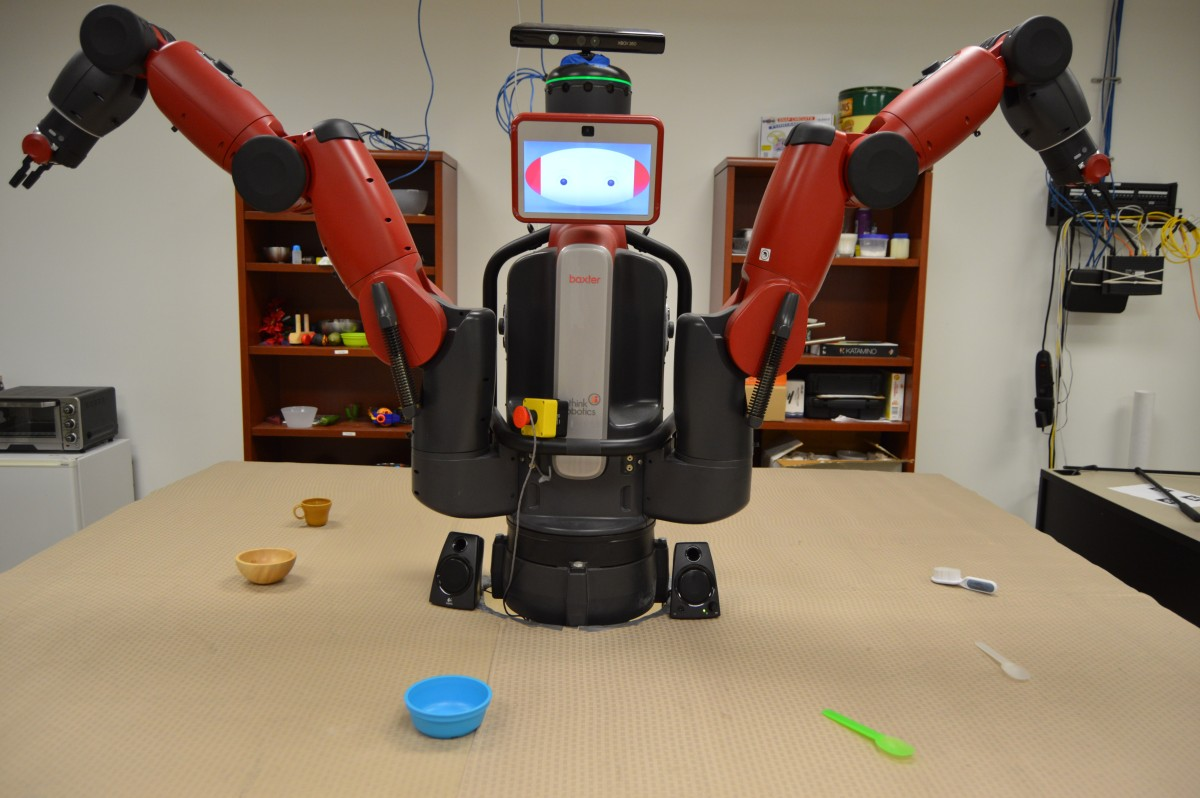
\includegraphics[width=1\linewidth]{figures/firstPerson.jpg}
\caption{\label{fig:firstPerson}The human's view when using our system to interact with the robot. The user and the robot participate in a conversation so that the robot can determine which of the
six objects the user desires. In counter-clockwise order the objects are: the brown mug, the wooden bowl, the blue bowl, the green spoon, the white spoon, and the white brush.}
\end{center}
\end{figure}
% no \IEEEPARstart
%In the future, personal robot collaborators will be ubiquitous assistants in the home. You will ask your robot to cook you a dish, and it will scan the Internet for thousands of recipes, interpret what it read, and use that information to cook better food. The human never needed touch a keyboard, or convert a recipe written for humans into something machine readable. My research aims to make this vision of the future of reality.

%This past school year, I wrote a paper realizing a small portion of that dream. Using a microphone and rgbd camera, a user was able to ask our robot to hand them the ingredients needed for a recipe. Our robot used the incoming speech data to infer the correct ingredient, and then place it in front of the user. As a baseline, or robot treated each hand-off as an independent event. Our contribution was a method where the robot used the history of past hand-offs to more accurately guess the desired ingredient.

% \stnote{This needs to follow the structure of the abstract but in more
%   detail.  The first paragraph about the problem, the next paragraph
%   about existing approaches and why they don't solve it.  Then a
%   paragraph or two about the approach you plan to use to solve it, and
%   how and why it works.  Finally a paragraph or two about how you plan
%   to evaluate or assess performance.}


When humans collaborate on a task---for example, repairing a car, or cooking a meal---both participants continually signal back and forth, communicating their current understanding of the task and the actions needed to achieve the goal. \citeauthor{clark96} describes communication as a \textit{joint activity}, similar to playing a duet or performing a waltz \cite{clark96}. In our work, we call this back and forth signaling \textit{social feedback}, and the goal is to use social feedback to improve the speed and accuracy of human-robot interactions. 

% \stnote{I saw the below note was commented out -- however we still
%   need this paragraph.  We can't just cite our work.  Please go and
%   read Bohus, Chai, and all of the papers cited in the ICMI reviews,
%   and write a paragraph contrasting us with related work.}

% \stnote{Need a paragraph about existing approaches that describes the
%   problem and why they fall short.}

Robotic research into establishing common ground is just beginning, but has already shown promise. In \cite{chai14}, they developed a system to establish new names for objects visible to the robot. \cite{williams15} describes an approach to understanding underlying semantics in human dialog. There are natural areas for improvement since both works rely on hand-coded rules or logical predicates, limiting easy expansion to new domains. 


%Currently, human-robot interaction has not taken full advantage of social feedback. \stnote{And also not true -- read Joyce Chai and Dan Bohus's work.  We should be citing them in the introduction.  }   In many cases, the robot is socially mute, unable to signal at all. Approaches that do use social feedback tend to focus on single domains, like speech, and often do not run in real time. 


%\stnote{Why are these notes commented out when they have not been addresed?}

 %\stnote{I wouldn't jump so quickly into object handoff.  Instead I
  % would try to get to the problem of generating feedback, and choosing
   %the appropriate action given the belief state.  I think object
   %handoff is one domain where we are demonstrating these ideas, but
   %not the only possible one, so let's save it for the evaluation.}

We propose an approach that will estimate the human's state and choose actions
in real time. Our system takes multimodal observations
as input, namely speech and gesture, and responds with speech according to a policy generated by solving a POMDP representation of the world.  We use an approximate solving technique
called Belief Sparse Sampling \cite{kearns02}. Performing inference is expensive, so we must
make optimizations to use the policy in real time, both in the model structure and by
caching the policy with k-nearest neighbors (KNN).


% We do this by assuming a human interprets a robot's
% actions in the same way the robot interprets a human's actions. Then we are
% able to reverse the Bayes filter we previously developed to generate actions
% that the human will understand. To choose the (approximately) optimal action,
% we will use a POMDP. POMDPs are useful for modeling this problem since they
% provide a systematic method of using memory of previous actions and
% observations to disambiguates the states of the world.


% \stnote{I would move object picking to here: to evaluat we focus on object
%  picking, where the robot is delivering an object to the person.}  



Our research focuses on an important part of physical
collaboration: object delivery. Object delivery is an
essential capability for robots~\cite{Huang15}. 
Our setup for object delivery is as follows: a human requests
a series of objects from the robot one at a time.  The human makes their
request using speech and gesture (pointing).  In previous work, the
robot had only two actions, deliver the object and wait. The robot collected
information from the human until its estimation of the desired object
crossed a threshold, then delivered the estimated object.  This
approach was successful if the observations were unambiguous to the
robot, but if the robot was unsure, it was unable to communicate that
fact to the human and could only wait passively for more information.
Our research provides a system that not only interprets the speech 
and gesture of the human to determine which object they desire, but 
also provides a flexible, non-rule based approach to dynamically generate
social feedback. 

Our model allows for incremental interpretation of speech and gesture, as implemented in our prior work. However, to circumvent practical issues in synchronizing human-robot dialogue, the robot waits until the human has finished each utterance before taking an action. Future work will focus heavily on adjusting our approach to appropriately handle barge-in by both human and robot. 
 
 
To evaluate our proposed approach, we conducted a user study where
participants asked for objects from the robot. We measured
speed and accuracy and compared the difference between trials that use
social feedback and trials that do not.


\begin{table*}
\begin{center}
\begin{tabular}{rl}
\toprule
 Variable & Explanation\\
\midrule
 $s = \langle \mathcal{O},\omega\rangle$ & A single state, which is made up of the given tuple \\
 $\mathcal{O} = \{x_1,...,x_D\}$ &  Set of all objects \\
 $\omega \in \mathcal{O}$ & Object desired by user \\
 $S = \{s_1 \dots s_N\}$ & Set of all states \\
 $x = \{name, vocab, position\}$ & An object, defined by a name, vocabulary, and position \\
 $a$ & A possible robot action. Speech and picking \\
 $A = \{a_1 \dots a_k\}$& Set of all robot actions \\
 $T(s, a, s^{t+1})=p(s^{t+1}|s^t,a^t)$& Transition function, probability of entering new state given current state and action \\
 $o = \langle l, g, \mathcal{O} \rangle$ & A single observation, made up of observed language, gesture, and objects \\
 $\Omega = \{o_1 \dots o_M\}$& Set of all possible observations \\
 $O(o^{t+1})=p(o^{t+1}|s^{t+1},a^t)$& Observation function, probability of an observation given the state and previous action \\
 $R(s,a) \in \mathbb{R}$& Reward function \\
 $\gamma \in [0,1]$ & Discount factor, discounts future rewards \\
\bottomrule
\end{tabular}
\caption{\label{table:variables}POMDP Variables.}
\end{center}
\end{table*}


\section{Related Work}
Work demonstrating the importance of social feedback in human-human
communication has been done in the field of psycholinguistics. In  \cite{clark04}, one human (labeled the builder)
builds a Lego model according to instructions given by another human
(labeled the director). In the feedback-free trials, the director's
instructions were prerecorded, and the resulting models were very
inaccurate (in fact no model was completely correct). In the feedback
trials, errors were reduced by a factor of eight. Our goal is to
enable a robot to collaborate with a human in this way.


Other work with collaborative robots exists, for example, \cite{foster12} have done research with a bar-tending robot. This robot follows a rule-based state estimator, and delivers drinks from fixed positions behind the bar to multiple users based on their speech and torso position. 
We expand the scope of the problem: we do not use a rule-based state planner, our items are not in fixed positions, and our gesture model uses pointing instead of torso position. 

In \cite{bohus14},  a robotic building guide directs guests to find specific rooms. Our project addresses a similar domain, requiring the interpretation of users' requests, but differs in the task and the type of communication necessary to accomplish that task. 

Other work involving robotic object delivery also exists. Some approaches have no social feedback and will either deliver the wrong item or do nothing if given a
request it does not understand~\cite{tellex11,matuszek12,tellex12,misra14}. Language only feedback models also 
exist~\cite{chai14,macmahon06,tellex11,matuszek12,guadarrama14,hewlett11,misra14}, and several gesture only models~\cite{waldherr00,marge11}.


\cite{matuszek14} shows promising work in fusing language and complex gesture to understand references to multiple objects at once. We build off this work by including social feedback. 

In the field of computational linguistics, previous work exists in resolving referring expressions incrementally, such as~\cite{schlangen09,kruijffincremental,Gieselmann}. Other work in that community also incorporates gesture, and/or eye gaze~\cite{kennington13,kennington15a}, but the given work does not incrementally update gesture along with speech. ~\cite{chairmi} provides work towards resolving referring expressions in a different domain, but does not address the task of acting on the results of these referring expressions. In~\cite{kruijffclarification}, they propose a system for planning to ask for clarifications, which covers a wide scope of knowledge failures. In this work, we are interested only in a small subset of these clarifications, and address the problem of how and when these clarifications should be used in a concrete human-robot collaboration task. 



% Despite demonstrations of social feedback's benefit to
% human-human interaction, current human-robot interaction does not fully
% exploit social feedback. For many approaches, the robot has no social feedback
% at all, and will either hand over the wrong item or do nothing if given a
% request it does not understand~\cite{tellex11, matuszek12, tellex12,
% misra14}. Approaches that do incorporate social feedback have focused on a
% single modality, usually language~\cite{macmahon06, tellex11, matuszek12,
% guadarrama14, hewlett11, misra14} and less often, gesture\cite{waldherr00,
% marge11}. Previous approaches with fused modalities~\cite{matuszek14} take
% many seconds to respond, diluting the benefit of the social feedback. Indeed,
% our groups previous research with social feedback only involved natural
% language and was not real-time~\cite{tellex12, deits13}.

POMDP approaches to dialog~\cite{young13} are quite common, but treat dialog
as a discrete, turn-taking interaction. The Dialog State Tracking
Challenge~\cite{williams2013dialog} a notable driving force for computer
dialog understanding, treats dialog in this turn-based way. Although the behavior of our system resembles turn-taking, our model treats dialogue as an incremental process and future implementations will make use of this. 


Alternative approaches to
POMDPs include cognitive architecutres such as SOAR~\cite{soar} or
DIARC~\cite{diarc}.  By taking a probabilistic approach, we can seemlessly
fuse information from multiple sources and explicitly reason about the
robot's uncertainty when choosing actions.

% We are unaware of
% any existing work that estimates mental states at the high frequencies
% necessary to produce continuous real-time social feedback.

%\stnote{Make sure we cite Joyce Chai and Dan Bohus, and the guy in the email I just sent.}

\section{Technical Approach}


The goal of our work is to enable the robot to correctly determine which object the human desires from their speech and gesture.

The robot might misinterpret a person's speech and gesture; to recover from these failures, the robot chooses speech actions of its own, which change the human's belief about what the robot knows, which in turn shapes the user's subsequent speech and gesture.
In actuality, we do not know how the robot's actions affect the human's belief or how the human's belief affects their subsequent actions. However, if we make certain assumptions about how the robot's actions affect what we observe from the human, we can formulate the model as a POMDP. 


%However, if we assume knowledge of how the robot's actions affect the human's state, the human's belief about the robot's knowledge becomes an observable variable, which reduces our belief space considerably. Because we now have our state factored into a fully observable and partially observable portions, we can use a Mixed Observability Markov Decision Process to represent our problem.


%The Bayes filter assumes an initial distribution (uniform), and at each timestep observes the human's speech and gesture. It integrates the observations over time, adjusting the belief distribution. We also need to alter the human's belief about what the robot will hand over. We can also accomplish this with a Bayes filter, by reversing its direction. Instead of the robot observing the human's speech and gesture, we model a human observing the robot's speech and gesture. In doing this make two assumptions. One, the initial distribution is uniform, and two, the human's belief updates are Bayesian. 


% \stnote{Need some introductory text framing describing the POMDP at a
%   high level.  Need to motivate pick-and-place as the sample domain,
%   and say at a high level what the states/actions are.}

\subsection{POMDP Overview}

To solve a POMDP, an agent must perform state-estimation and policy generation. The state estimator calculates a belief state, which is a probability density function (pdf) over all possible states, and the policy generator chooses an action that maximizes the agents expected cumulative reward according to a given reward function. 

\subsubsection{State Estimator}
The state estimator assumes an initial belief, and uses Bayesian mathematics to update its belief over time. In order to perform this update, the state estimator has a model of how the true state emits observations and how actions affect the state. These two models are called the observation function and the transition function.


\subsubsection{Policy Generator}
The policy generator chooses a set of actions that maximizes the expected value of its reward over time. The reward for a state-action pair is given by a reward function.  
%For our chosen problem, the robot must estimate the human's desired object as quickly and accurately as possible. To do this, the robot can observe the humans actions, and respond to them with questions, statements, and gestures that explain to the human the robots internal belief. This problem is symmetrical. Both actors have the same set of actions and observations, and share a common goal. A Bayes filter is a good choice for estimating the states, as they are fast, allow for multiple observation sources, and are generative. Being generative is good, as it allows for the model be reversed, something expanded on below. 

\subsection{POMDP Definition}
We define our POMDP by the tuple \{$S, A, T, R, \Omega, O$\}.


%\stnote{I think we should call it a mixed observable Markov Decision Process.}

\begin{itemize}

	\item $S$ is the set of states. In this problem, a state is a tuple of two items $\langle \mathcal{O}, \omega \rangle$. $\mathcal{O}$ is the is the set of objects available for the robot to deliver. Each element $x \in \mathcal{O}$ is an object with a name, unigram vocabulary, and position. An example value $\mathcal{O}$ could be the set of objects \{redBowl, greenSpoon\}.  An example $x \in \mathcal{O}$  for a red bowl would be (redBowl, \{red, bowl, plastic\}, (1.0, 2.0, 0.0)). The object the human desires is denoted $\omega \in \mathcal{O}$. While $\mathcal{O}$ is considered a known variable, $\omega$ is hidden, making our POMDP a Mixed Observability MDP~\cite{momdp}
	\item $A$ is the set of actions. The robot can deliver an object, do nothing, or ask a question about a property of the desired object. 
	\item $T = p(s^{t+1}|s^{t},a^{t})$ is the transition function. It calculates the probability of transitioning from the current state to the next state given the current state and current action. We make the assumption that the human participant does not change the object they desire unless their object is successfully delivered. 

	\item $R$ is the reward function. The reward function  takes as input a state and action, and gives a real-valued reward. 
		The reward for delivering the correct object is $10$ whereas delivering the incorrect object yields a penalty of $-80$ because it can have negative side effects and is time consuming. Doing nothing yields $-1$ as a penalty for time passing. Talking yields $-4$ to penalize bothering the user. These values were chosen empirically and have a natural interpretation when considered relative to the penalty for time passing. 
		
  \item $\Omega$ is the set of possible observations, $\langle l, g,\mathcal{O}\rangle \in \Omega$.  $l$ is the human's speech, $g$ is the human's gesture, $\mathcal{O}$ is as defined above.  
  \item $O = p(o^{t+1}|s^{t+1},a^t)$ is the observation function which describes how states emit language and gesture from the human. 
  
  %\stnote{It should be $\omega \in \mathcal{O}$ }
  %\stnote{No unbound this}
  %\stnote{Let's just call it s and g.} 
  %\stnote{We should say it includes a pose as well as object proporties.}
  %We assume conditional independence for speech and gesture, so we can factor the equation to be $O(o_{s_{t+1}}|s_{t+1},a_t) (o_{g_{t+1}}|s_{t+1},a_t)$ %\stnote{Can you write this as a probability using the tuple representation for $o$?}
  %\item $b_o$ is the belief state of the desired object. This is a distribution modeling what the robot thinks the human wants.
  %\item $b_h$ is the belief state of what the human thinks the robot thinks the human wants. We want this to be as close as possible to $B_h$. \stnote{I wouldn't say ``we want''; this should be coming from the reward function, so it should be defined there.}
\end{itemize}


\begin{figure}[h]
\centering
\resizebox{0.3\textwidth}{!}{%
	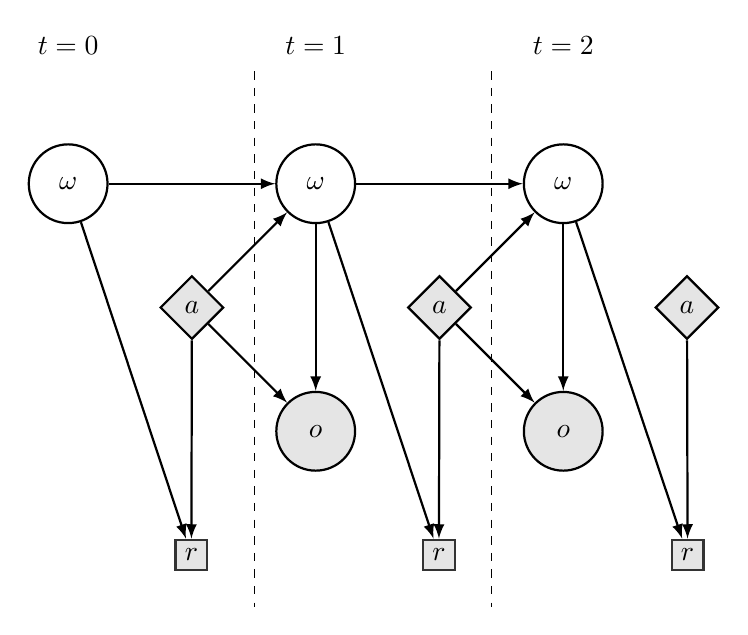
\begin{tikzpicture}
	\tikzstyle{main}=[circle, minimum size = 10mm, thick, draw =black!100]%, node distance = 8mm]
\tikzstyle{action}=[diamond, thick, draw =black!100]
\tikzstyle{connect}=[-latex, thick]
\tikzstyle{box}=[rectangle, draw=black!100]
  %\node[main, fill = white!100, draw =white!100] (o) {};
  \node[action, fill = black!10] (a)  {$a$};
  \node[main, fill = white!100] (s_o)[above left = of a] {$\omega$};
  \node[main, fill = white!100] (s_o2) [above right= of a] {$\omega$};
  \node[main, fill = black!10] (o2) [below right=of a] {$o$};
  \node[action, fill = black!10] (a2) [above right=of o2] {$a$};
  \node[main, fill = white!100] (s_o3) [above right= of a2] {$\omega$};
  \node[main, fill = black!10] (o3) [below right=of a2] {$o$};
  \node[action, fill = black!10] (a3) [below right=of s_o3] {$a$};


  \node[rectangle, thick, draw=black!80, fill=black!10] (r1) [below left=of o2] {$r$};
  \node[rectangle, thick, draw=black!80, fill=black!10] (r2) [ below left=of o3] {$r$};
  \node[rectangle, thick, draw=black!80, fill=black!10] (r3) [below right=of o3] {$r$};

  \path (s_o) edge [connect] (s_o2)
		(s_o2) edge [connect] (s_o3)
		(a) edge [connect] (s_o2)
		(a2) edge [connect] (s_o3)
		(s_o2) edge [connect] (o2)
		(s_o3) edge [connect] (o3)
		(s_o) edge [connect] (r1)
		(a) edge [connect] (r1)
		(a) edge [connect] (o2)
		(s_o2) edge [connect] (r2)
		(a2) edge [connect] (r2)
		(a2) edge [connect] (o3)
		(a3) edge [connect] (r3)
		(s_o3) edge [connect] (r3);
  \draw [dashed] (0.8,3) -- (0.8,-3.8);
  \draw [dashed] (3.8,3) -- (3.8,-3.8);
  \node [above= 1cm of s_o] {$t=0$};
  \node [above= 1cm of s_o2] {$t=1$};
  \node [above= 1cm of s_o3] {$t=2$};
  \end{tikzpicture}
  }
\caption{\label{fig:pomdp_graphical_model}Graphical model of proposed POMDP over three timesteps. Gray nodes are observable.}
\end{figure}

A concise list of the POMDP variables is shown in Table~\ref{table:variables}.

\subsubsection{Observation Function}

The observation function calculates the probability of an observation given the state and previous action. 

\begin{equation}\label{eq:of_def}
O(o^{t+1},s^{t+1},a^t) = p(o^{t+1}|s^{t+1},a^t)
\end{equation}

We can expand Equation~\ref{eq:of_def}.

%\stnote{Really this is rewriting it substituting in the observation and state functions; you haven't factored yet.}

%\stnote{This math is wrong; it should be $\mathcal{O}$ and not $\sigma$.}

\begin{equation}\label{eq:of_factor}
	O(o^{t+1}) = p(\mathcal{O}^{t+1},l^{t+1}, g^{t+1}|\mathcal{O}^{t+1},\omega^{t+1}, a^t)
\end{equation}

The set of objects on the table is only dependent on itself, so we can now factor Equation~\ref{eq:of_def} to separate $\mathcal{O}$.

\begin{equation}\label{eq:of_factor2}
O(o^{t+1}) = p(\mathcal{O}^{t+1}|\mathcal{O}^{t+1})p(l^{t+1}, g^{t+1}|\mathcal{O}^{t+1},\omega^{t+1}, a^t)
\end{equation}

In our problem we assume no error in observing $\mathcal{O}$. Therefore the first term is equal to one. We can simplify and remove it from the equation.

\begin{equation}\label{eq:of_factor_simple}
O(o^{t+1}) = p(l^{t+1}, g^{t+1}|\mathcal{O}^{t+1},\omega^{t+1},a^t)
\end{equation}

If we assume conditional independence of speech and gesture, we can factor
Equation~\ref{eq:of_factor_simple} one step further.  Conditional independence
in this case means that, conditioned on the object that the user desires, the
speech and gesture observations are independent of each other. 

\begin{equation}
	O(o^{t+1}) = p(l^{t+1}|\mathcal{O}^{t+1},\omega^{t+1},a^t)p(g^{t+1}|\mathcal{O}^{t+1},\omega^{t+1},a^t)
\end{equation}

It may seem inaccurate to assume speech and gesture are conditionally independent, but empirically, we observe that when the true state is known, language and gesture are largely but not completely independent. This assumption simplifies our model and allows us to separate the observation function into a language model and a gesture model. 

\subsubsection{Language model}
In the language model, we observe two types of speech: General speech is interpreted according to a unigram model, while yes/no responses are handled separately. 

For most speech input, we use a unigram model. For each word in the observed speech, we calculate the probability that, given the state, that word would have been used to describe the state. We assume here that $\mathcal{O}$, the set of objects available, does not affect which words the participant would speak, though in practice, humans do tailor their speech in response to different objects. 

\begin{align*}
	p(l^{t+1}|\mathcal{O}^{t+1},&\omega^{t+1},a^t)\\
	&= p(l^{t+1}|\omega^{t+1},a^t)  \\
	&= p(c|\omega^{t+1}, a^t)\prod_{w \in l^{t+1}} p(w|\omega^{t+1},a^t)
\end{align*}


Where $p(c|\omega^{t+1},a^t)$ describes the probability that the human chooses to communicate given the state and action. We assume that this is independent of $\omega$, and depends only on the action; if the robot asks a question, the human is more likely to respond: 
\begin{equation}
	p(c|a^t) = \begin{cases}
		0.8 & \text{if $a^t$ is a question} \\
		0.2 & \text{otherwise}
	\end{cases}
\end{equation}

The probability of a particular word being used to describe a particular object is determined by consulting the object's vocabulary. Specifically, 

$$p(w|\omega^{t+1}, a^t) = \frac{\text{Number of times $w$ is used to describe $\omega$}}{ \text{Total counts for words describing $\omega$}}$$


If $w$ is not part of the object's vocabulary, we assign it a small probability $\epsilon$. 

While a unigram model is rudimentary, it serves as a good starting point for our work and produces adequately accurate results. In the future, more sophisticated language models will be considered. 

The user may also say ``yes'' or ``no'' in response to a question that the robot has asked, in which case we handle the utterance differently. In the case where the robot has not asked a question, the probability of the user answering ``yes'' or ``no'' is assigned probability $\epsilon$. If the robot has asked a question, 
\begin{align*}
	p(l^{t+1} &= ``yes" | \mathcal{O}^{t+1}, \omega^{t+1}, a^t)  \\
	&= p(c|a^t)p(l^{t+1} = ``yes" | \omega^{t+1}, a^t) 
\end{align*}

\begin{equation}
	p(l^{t+1} = ``yes" | \omega^{t+1}, a^t) = \begin{cases}
		1  & \text{if  $a^t.\text{text} \in \omega.\text{vocab}$} \\
		0  & \text{otherwise}
	\end{cases}
\end{equation}


\begin{align*}
	p(l^{t+1} &= ``no" | \mathcal{O}^{t+1}, \omega^{t+1}, a^t)  \\
	&= p(c|a^t)p(l^{t+1} = ``no" | \omega^{t+1}, a^t) 
\end{align*}

\begin{equation}
	p(l^{t+1}=``no" | \omega^{t+1}, a^t) = \begin{cases}
		0  & \text{if  $a^t.\text{text} \in \omega.\text{vocab}$} \\
		1  & \text{otherwise}
	\end{cases}
\end{equation}

We assume that the probability the user says ``yes'' or ``no'' is independent of $\mathcal{O}$.

In addition, to account for the user not answering quickly enough, the state includes the the last question asked by the robot.


\subsubsection{Gesture Model}
The gesture model operates on the vector defined by the participant's shoulder and hand, called $v_t$. The intersection of $v_t$ with the plane of the table is considered to be the target of the pointing gesture, $p_t$. We assume the participant samples this point from a 2 dimensional Gaussian distribution centered at the location of the object the
participant is indicating, with a hand-chosen variance $\sigma$. Therefore, the probability of a gesture given a state
is as follows: 

\begin{align}
	p(g^{t+1}|\mathcal{O}^{t+1},&\omega^{t+1},a^t)\\
	&= p(g^{t+1}|\omega^{t+1})  \\
   &\propto \mathcal{N}(\mu = (\omega.x, \omega.y), \sigma)[(p_t.x, p_t.y)]
\end{align}


Again we assume that the gesture the participant chooses is independent of the other objects on the table and their placement, though this is not the case in practice. 


We also track an additional vector called $u_{t,x}$ defined by the angle between the participant's shoulder and an object $x\in \mathcal{O}$. 
For each $x \in \mathcal{O}$, we calculate the angle between $v_t$ and $u_{t,x}$. If the smallest angle is over a certain threshold, then no gesture was performed and the term is not factored into the overall observation model. 


%\stnote{I think there is one more term where you assume observations
%  are conditionally independent given the state.}

\subsubsection{Transition Function}
The transition function calculates the probability of moving to a particular new state given 
the current state and action.

\begin{equation}\label{tf_def}
T(s^{t+1},s^t,a^t) = p(s^{t+1}|s^t,a^t)
\end{equation}

We substitute the corresponding variables into (\ref{tf_def}).

\begin{equation}\label{tf_def_expanded}
T(s^{t+1}) = p(\mathcal{O}^{t+1},\omega^{t+1}|\mathcal{O}^{t},\omega^{t},a^t)
\end{equation}

The set of desired objects on the table and the desired object only depend on themselves and the last action taken, so we can factor (\ref{tf_def_expanded}).

\begin{equation}\label{tf_factored}
	T(s^{t+1}) = p(\mathcal{O}^{t+1}|\mathcal{O}^{t}, a^t)p(\omega^{t+1}|\omega^{t}, a^t)
\end{equation}

The two terms from (\ref{tf_factored}) have simple stepwise functions if $a^t$ is not a pick action. 

\begin{equation}
	p(\mathcal{O}^{t+1}|\mathcal{O}^{t}, a^t) = 
\begin{cases} 
	1 & \text{if } \mathcal{O}^{t+1} = \mathcal{O}^t \\
  0 & otherwise
\end{cases}
\end{equation}

\begin{equation}
	p(\omega^{t+1}|\omega^{t}, a^t) = 
\begin{cases} 
	1 & \text{if } \omega^{t+1} = \omega^t \\
  0 & otherwise
\end{cases}
\end{equation}

If $a^t$ is a pick action, the transition model for $\mathcal{O}$ is defined as follows: 

\begin{equation}
	p(\mathcal{O}^{t+1}|\mathcal{O}^{t}, a^t) = 
\begin{cases} 
	1 & \text{if } \mathcal{O}^{t+1} = \mathcal{O}^t \setminus \{a^t.\text{object}\} \\
  0 & otherwise
\end{cases}
\end{equation}

If $a^t$ is a pick action and the user's desired object $\omega$ is picked, $\omega$ transitions as follows. 

\begin{equation}
	p(\omega^{t+1}|\omega^{t}, a^t) = 
\begin{cases} 
	0 & \text{if } \omega^{t+1} = \omega^t \\
	1/|\mathcal{O}^{t+1}|	& otherwise
\end{cases}
\end{equation}

Otherwise, it is the same as if some other action had been taken.


\subsubsection{Actions}

The robot must choose among the actions available to it. With social feedback enabled, these actions are: 
\begin{itemize}
	\item Pick up an object and deliver to the human
  \item Ask a question of the form ``Would you like a \emph{$\langle$object property$\rangle$} object?''
  \item Wait (do nothing)
\end{itemize}

With social feedback disabled as in the baseline, these actions are: 
\begin{itemize}
	\item Pick up an object and deliver it to the human
  \item Wait (do nothing)
\end{itemize}

Asking a question serves both as an information gathering action (as it prompts
the human to respond with additional information) and also a means for the
robot to express its uncertainty about which object is desired. These questions
directly mirror the unigram model of speech that we use to interpret human
language, i.e., each question asks about a one-word property of the object,
such as its color (e.g., blue), material (e.g., wooden) , or noun description
(e.g., cup). Asking about a particular property allows the robot to reference
all objects with that property at the same time. An additional benefit of using
this simple question format is that if we assume the human interprets speech
with the same model as the robot, its effect on its belief about the robot's
knowledge is easy to predict.  We will explore this in future work. 

We also give the robot the action to do nothing for a given timestep. This is
important in preventing the robot from inundating the human with speech
utterances. 

\subsection{Policy Generation}


%Controlling a MOMDP can be broken into two parts: estimating the state, and generating actions. A MOMDP agent keeps an internal belief state $b$, which it generates and updates with a state estimator. $b$ is not a single state, but rather distribution over possible state. In our case, our belief state is $b(s')$, which tracks $s'$.   

%\begin{equation}\label{belief_omega}
%b(s') = p(s'|o,a,b)
%\end{equation}

%\stnote{Can you write it as a probability?  I'd like to see an equation here.}


The optimal policy can be exactly calculated, but is intractable due
to the size of the state space. Fortunately, approximate solutions
exist. Currently, a representation of this POMDP has been specified
with the Brown-UMBC Reinforcement Learning and Planning (BURLAP) library\cite{burlap}, a
learning and planning library that can solve POMDPs.  For a solver, we use  Belief Sparse Sampling, a finite horizon
planning algorithm used on the POMDP's belief MDP that allows us to specify how deep to search and the number of observations to sample at each timestep. 


However, even using Belief Sparse Sampling, it was still not fast enough to allow the robot to respond in real time. As the number of objects grows, the number of states and the number of actions needed to address those states grow. For example, adding 1 additional object increases the number of states by 1 but increases the number of actions from anywhere between 1 (1 additional pick action) to several dozen (1 for each new unigram description of the object in its vocabulary). Each of these contributes to the branching factor, causing the the computation to quickly grow intractable even with a limited search depth. 

In big-O notation, the runtime of calculating the next decision can be expressed as $O((s*a*o)^d)$, where $s$ is the number of states, $a$ is the number of actions, $o$ is the number of sampled observations, and $d$ is the search depth. We can rewrite $a$ as $a = s + h*s+ 1$, because we have 1 pick action per state, some constant number $h$ property questions for each object, and one wait action. $o$ and $d$ are both chosen as constants, which gives a big-O runtime of $O((s^2)^d)$. 




We combat this exponential growth by limiting the number of actions per object to 2 (which should be enough for the robot to express which object it is referring to) as well as condensing the pick actions into a single macro action. This macro pick action allows the robot to pick the object with the greatest belief, and saves it from considering pick actions that are likely to be incorrect. Our new run time is $O((s*a*o)^d)$ where $a = 1 + 2s + 1$ (1 macro pick action, at most 2 question actions per state, and 1 wait action). While the big-O runtime remains the same, the improvement to constant factors is significant when adding new objects to the domain. 



Even with these measures to reduce the branching factor, the system did not run fast enough for real time at the search depth needed for meaningful decisions. In order to obtain real time responses, we run a simulated environment of our domain, with simulated object locations and simulated user input. We cached the results of several thousand decisions made by Belief Sparse Sampling, storing the belief state and the action chosen. Then, at interaction time, we use these results to make a decision about which action to take. Specifically, we perform a KNN classification where the feature vector is composed of the belief values of the POMDP's belief state and the class label is the chosen action. At runtime, we are given an input vector of the current belief state, which we classify and then perform the action given by the class label. This allows for nearly instantaneous responses, enabling us to make real time decisions. 

Making these optimizations is not ideal. For example, adding or changing the set of objects on the table requires rebuilding the KNN cache.  In the future we will likely move to alternative POMDP solvers which should give better performance. 

%\stnote{We should know if one of these solvers would work; I don't think we've tried any of them yet.  So listing them doesn't help much.  It might be worth talking to Nakul about this.}

% \subsection{Robot Feedback}

% Due to the structure of the MOMDP/POMDP, the robot will try to make $b_h$ be identical to $b_o$. This is desirable as this will reduce errors. If the robot thinks the human wants object A, the robot will point to/speak about object A to make $b_h$ and $b_o$ match (see Figure~\ref{fig:gesture_example}).

% \begin{figure}[h]
% \centering
% \begin{tikzpicture}%[trim axis left, trim axis right]
% \begin{axis}[ 
% ybar,
% enlarge x limits=0.4,
% %height=5.0cm, 
% width=0.4\textwidth,
% ylabel={Probability},
% xlabel={Objects}, 
% symbolic x coords={A, B, C},
% xtick=data,
% ymax=1.1
% ]
% \addplot coordinates {(B,0.0) (A,1.0) (C, 0.0)};
% \addplot[red,fill = red!10] coordinates {(B,0.33) (A,0.33) (C, 0.33)};
% \addplot[red,fill = red!40] coordinates {(B,0.05) (A,0.9) (C, 0.05)};
% \addlegendentry{$b_o$}
% \addlegendentry{Initial $b_h$}
% \addlegendentry{Final $b_h$}
% \end{axis}
% \end{tikzpicture}
% \caption{Using social feedback to match $b_o$ and $b_h$. Initially $b_o$ is weighted towards object A while $b_h$ does not, so the robot speaks and/or gestures towards object A, more closely aligning the two distributions.}
% \label{fig:gesture_example}
% \end{figure}

% We can calculate the difference between $b_o$ and $b_h$ using KL divergence. 

\section{Evaluation}
We evaluated the POMDP with social feedback against a baseline system
which is unable to speak and only able to listen. Each system was evaluated
by six users. We report four metrics: the number of picks that delivered the correct object (picks correct), the number of total attempted picks, the average time from the end of the first utterance referring to an object
until the end of the delivery of that object (EUED time), and the fractional amount of time spent delivering an incorrect object (IOD time).

\subsection{User Study Protocol}
Participants for this user study were acquired through convenience sampling by
inviting volunteers from the Brown University CIT building and the campus area
surrounding it. We gathered 6 participants. Each participant
contributed two trials, a baseline trial and a social feedback trial. During
the baseline trials, all feedback from the robot was excluded. During the
social feedback trials, the robot communicated with the participants through
voice and animated eye gaze which indicated the directions of the objects. The
order of these two trials was randomly assigned to each participant.
 
The participants interacted with a modified Baxter robot to perform a pick
and place task with six everyday objects: a brown mug, a wooden bowl, a blue
bowl, a green spoon, a white spoon, and a white brush. The six objects were
placed on a large table, behind which the robot was stationary. The six
objects and their starting locations stayed unchanged for all participants.

At the beginning of each study, the user was given a headset microphone,
calibrated the Kinect, and faced Baxter (Figure~\ref{fig:firstPerson}). The
headset microphone left their arms free to gesture.  They were instructed to
choose an object on one side of the table and then to indicate the desired
object through a combination of pointing and natural language
instructions. They were told to continue indicating until the desired object had been 
delivered. If the robot delivered an incorrect object, the user continued
interacting until the correct object was delivered. Next they were instructed to
do the same for an object on the other side of the table. Once the second
object was delivered, the user was finished with the first half of the study. 

Each participant first completed the above study with social feedback either
disabled (baseline) or enabled.  The participants were then given a follow up
survey to record their subjective reactions towards the robot. The survey
measured the participants' impressions on the robot concerning its level
of friendliness, reliability, capability, communication skills and their
perception of safety.  After the survey, the participant completed a second
study with social feedback either enabled or disabled, so that after the
second study the participant had completed the trial once with feedback on and once with
feedback off. Half the participants tried with feedback first.  After the
second trial, the user was dismissed.  There were no trials where the first
object delivery left no objects on the opposite side.

We expect to continue the survey as part of ongoing research to 
support our exploration of  human-robot interaction. The detailed results and
analysis of this survey will be included in our future studies.

\subsection{Results}

The results of our user studies are summarized in
Table~\ref{table:expResults}.  When using social feedback we observed a four
second average decrease in the EUED time but we incurred one additional
incorrect pick. Since we performed a statistically small number of trials, we
view these results more as a proof of concept than as a rigorous evaluation. 

\begin{table}
\begin{center}
\begin{tabular}{lrr}
\toprule
Metric & No Feedback & Feedback \\
\midrule
Picks Correct & 12/13 & 12/14\\
EUED Time & 17.33s & 13.33s\\
IOD Time & 2.59\% & 3.18\%\\
\bottomrule
\end{tabular}
\caption{\label{table:expResults} Experimental Results. EUED time is time from
the end of the first utterance in the request until the end of delivery of the
desired object and IOD time is time spent delivering incorrect objects.}
\end{center}
\end{table}

\subsection{Discussion}


Social feedback enables logical conversations between human and robot which allow the
robot to quickly determine the user's object of choice (Table~\ref{table:expDialogue}). 
In the first example, the user indicates that they want a spoon. This is an ambiguous statement
because there are two spoons, one of them white and the other green. The model can capture
the fact that asking about the color of the spoon will determine the object. The robot asks
if the user wants a white object, and when the user indicates that they do not, the robot
knows that the object in question is the green spoon. Similarly, wanting a bowl is ambiguous
because there is a blue bowl and a wooden bowl, so the robot asks about the color of the
object, determining that the user wants the blue bowl. This type of inference is not limited to
speech: ambiguous gestures can be resolved by asking about one of the candidate objects, as in the
case of the wooden bowl and brown mug.

By asking questions, the agent divides and conquers the belief space. Constructing
a POMDP for an arbitrary set of objects is easier than specifying search rules
in multimodal interaction spaces with complicated relationships between objects.
Solving a POMDP allows those rules to be discovered rather than specified, and the
burden is transferred from the modeler to the solver.




\begin{table}
\begin{center}
	\scalebox{0.95}{
\begin{tabular}{lr}
\toprule
Human & Robot \\
\midrule
I want a spoon. & \\
 & Would you like a white object?\\
No. & \\
 & (Picks the green spoon.)\\
\midrule
I want a bowl. & \\
 & Would you like a blue object?\\
 Yes. & \\
 & (Picks the blue bowl.)\\
\midrule
(Points ambiguously at & \\
the wooden bowl & \\
and brown mug.) & \\
 & Do you want the cup?\\
No. & \\
 & (Picks the wooden bowl.)\\
\bottomrule
\end{tabular}
}
\caption{\label{table:expDialogue} Example dialogue from interactions with our system. The robot chooses to ask more informative questions because the search depth of the planner is three rather than two.}
\end{center}
\end{table}

Without social feedback,
users must resort to repeating instructions with no idea whether their input is
received by the robot or whether it is interpreted correctly. This might lead
to frustration and a lower long term tolerance of the system.  When the robot
can reason about and issue social feedback and tell the user what it believes,
the user and the robot can engage in a natural dialogue which quickly
determines the item of choice. We predict that because the interaction is more
like a human-human interaction, users will be able to engage with the system for longer periods
of time with less frustration.
 

\section{Conclusion}

Social feedback is key to human-human interaction. This research
hopes to give robots the ability to participate in social feedback, making
human-robot interaction easier, faster, and more accurate. Our approach uses a
POMDP that takes input from a human in the form of speech and
gesture, estimates the human's mental state, and chooses
social feedback actions to facilitate the determination of the desired object.  
Our results suggest that by incorporating social feedback we can expect a decrease
in response time, but more experimentation is required.

\subsection{Future Work}

We plan to expand our current approach by implementing robotic gesture as an
additional feedback action the robot can take. This will add to the the number
of actions and make planning more expensive, but by implementing robotic speech
and gesture as collapsed actions similarly to our pick action, we should
maintain computational tractability. Moving beyond a unigram speech model would
allow more sophisticated references involving multiple objects, such as ``the
bowl behind the spoon.''  Finally, a placement action would allow us to
support more complex collaborative tasks.

In addition, we would like to explore the potential for richer communication
by having the robot track the human's belief about its current state. Adding this 
additional state variable would greatly increase the computational complexity of 
this task, but also allow it to make decisions that consider how its actions are 
perceived by the human. 


\subsection{Acknowledgment}

This paper is a collaboration between Brown University's Humans to Robots Laboratory and the Rhode Island School of Design's Industrial Design department. We would like to thank Dr. Claudia B. R\'{e}bola, associate professor at the Rhode Island School of Design, for organizing this collaboration and providing valuable guidance in designing the user experience and conducting user studies. 


This work was in part supported by the National Science Foundation under
``NRI: Collaborative: Jointly Learning Language and Affordances,'' grant \#
ISS-1426452.  It was also supported by the Army Robotics CTA under
``Robotics CTA: Perception, Human-Robot Interaction,'' grant \# 40228388.


\bibliographystyle{aaai}
\bibliography{main}
%\bibliography{references,main}

\end{document}

